
\subsection{Création de scènes plus complexes}
Nous avons commencé à faire des scènes plus complexes, avec différentes géométries, différentes transformations et plusieurs couleurs afin de tester les capacités du moteur. Le but était également de créer une scène qui puisse être agréable à regarder et qui permette de montrer ce que l'on peut faire avec ce moteur.\\ 
\par
Nous avons également ajouté un ciel plus réaliste, qui rougit lorsque le soleil est bas sur l'horizon. Les composantes vertes et bleues de la couleur du ciel sont multipliées par le produit scalaire avec la direction des rayons du soleil.\\
Ainsi, il ne reste plus que le rouge lorsque le soleil s'approche de l'horizon.
\begin{figure}[h]
    \centering
    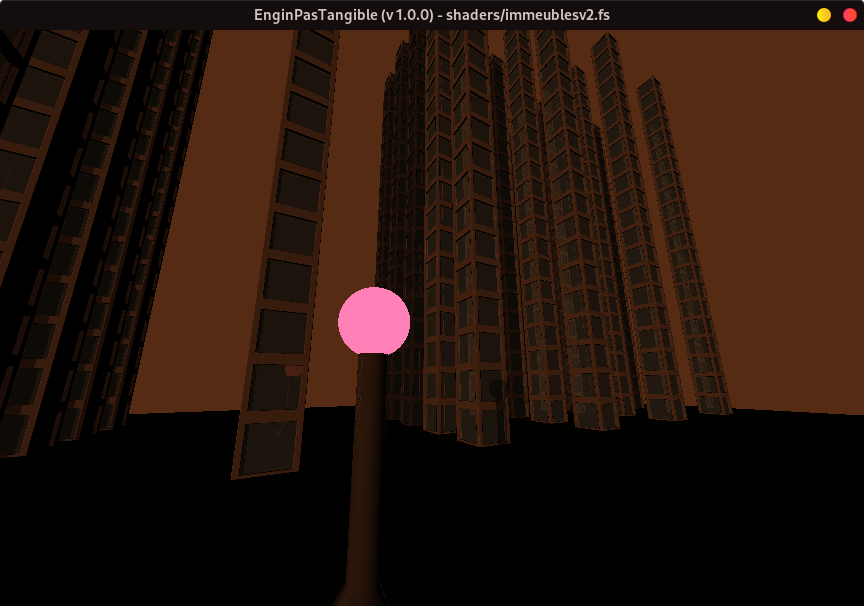
\includegraphics[width=7cm]{images/screens/ville1matin.png}
    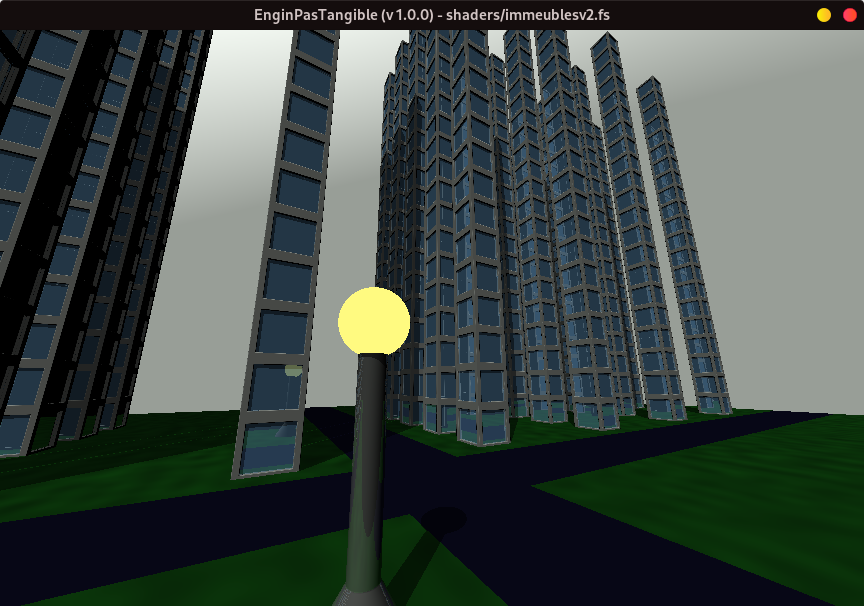
\includegraphics[width=7cm]{images/screens/ville2jour.png}
    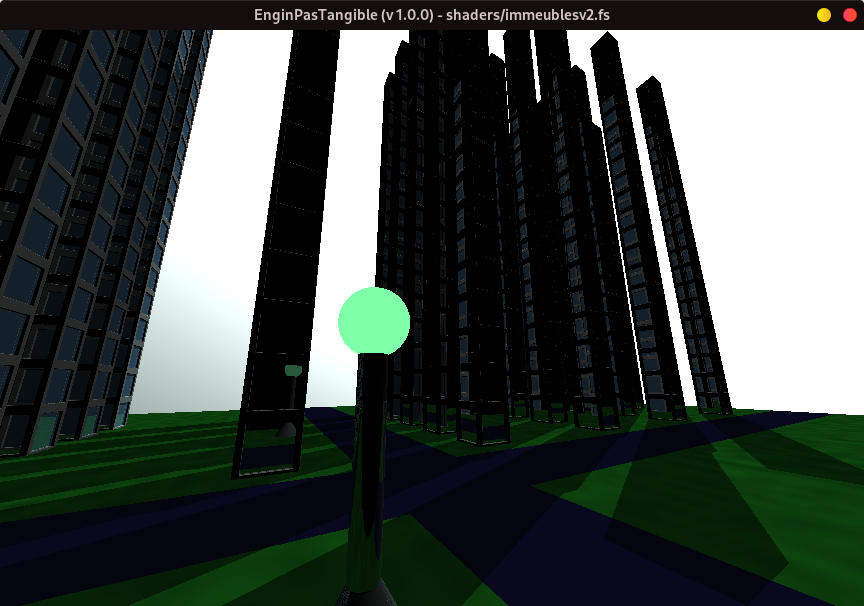
\includegraphics[width=7cm]{images/screens/ville3aprem.png}
    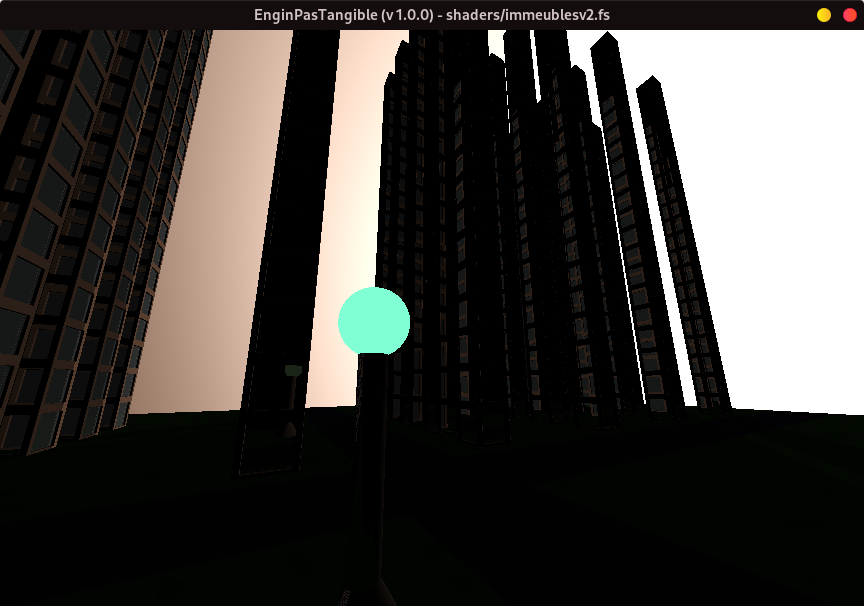
\includegraphics[width=7cm]{images/screens/ville4soir.png}
    \caption{Scène avec des immeubles et un cycle jour/nuit}
    \label{fig:city}
\end{figure}

